\begin{figure}[h!]
    \centering
    \caption{Randomization Inference for the Direct and Spillover Effects of \emph{Plan Cuadrante}}
    \label{fig:ri_placebo}
    \begin{subfigure}{0.495\textwidth}
        \centering
        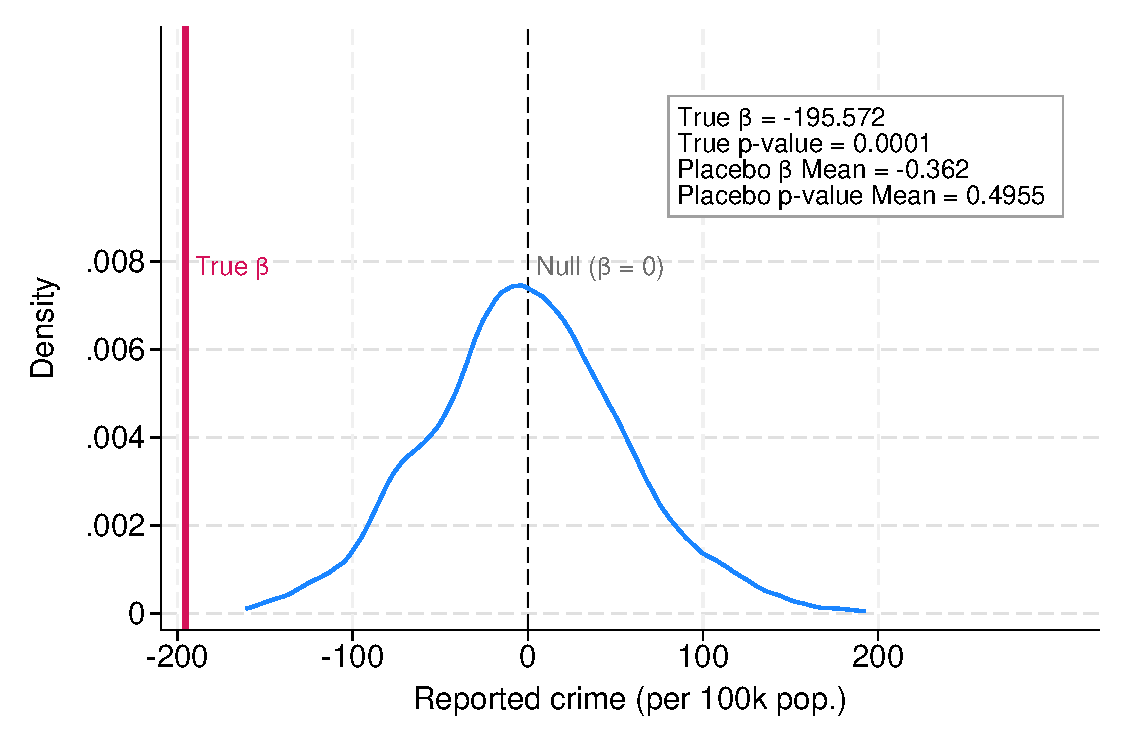
\includegraphics[width=\textwidth]{../manuscript/Graphs/CHDH_RI_placebo_crime.pdf}
        \caption{Reported crime}
        \label{fig:ri_crime}
    \end{subfigure}%
    ~
    \begin{subfigure}{0.495\textwidth}
        \centering
        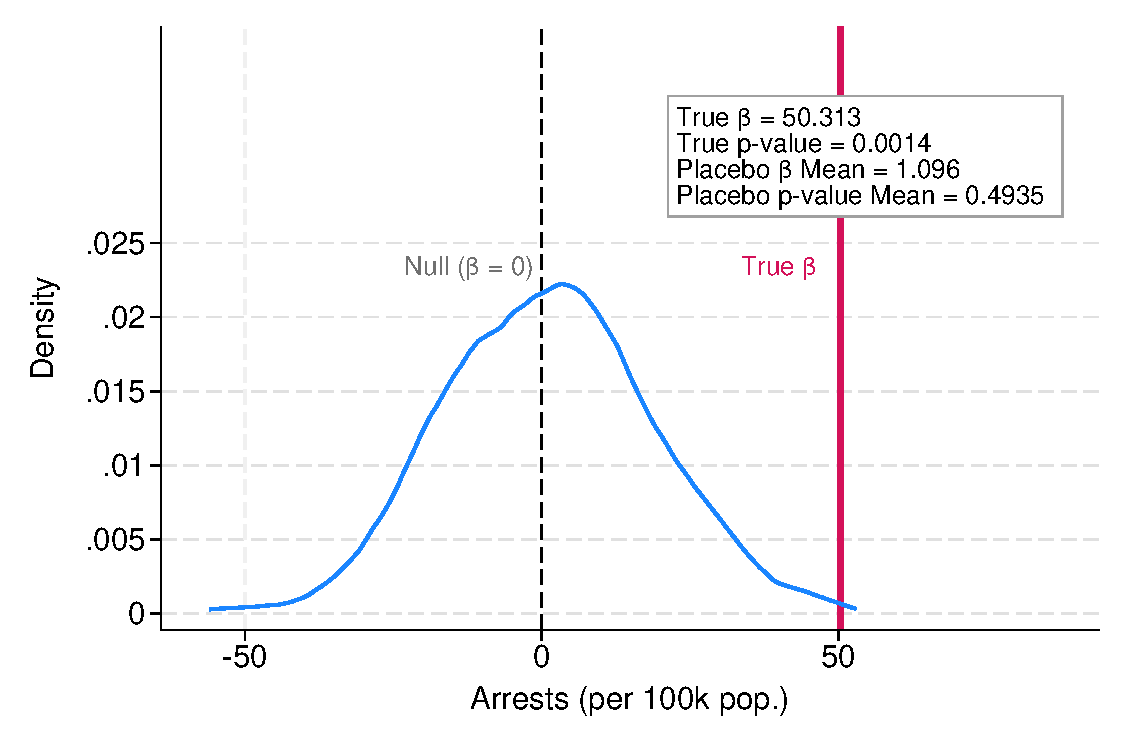
\includegraphics[width=\textwidth]{../manuscript/Graphs/CHDH_RI_placebo_arrests.pdf}
        \caption{Arrests}
        \label{fig:ri_arrests}
    \end{subfigure}

    \begin{subfigure}{0.495\textwidth}
        \centering
        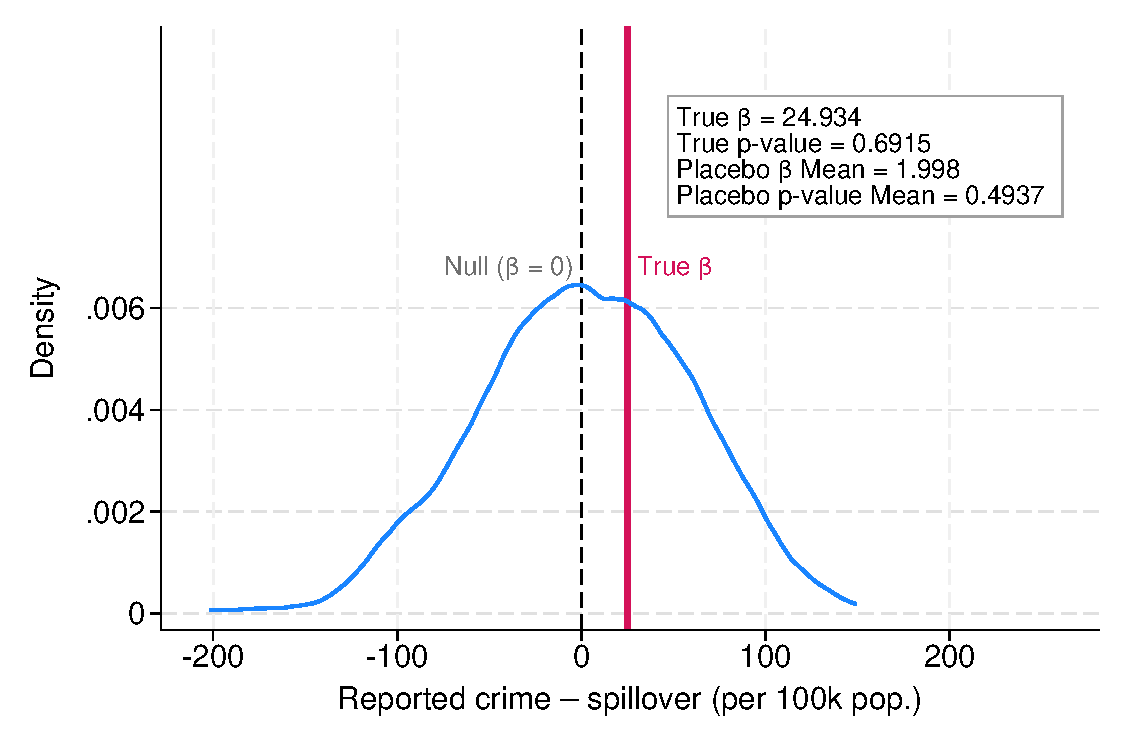
\includegraphics[width=\textwidth]{../manuscript/Graphs/CHDH_RI_placebo_crime_spillover.pdf}
        \caption{Spillovers on Reported crime}
        \label{fig:ri_crime_spillover}
    \end{subfigure}%
    \begin{subfigure}{0.495\textwidth}
        \centering
        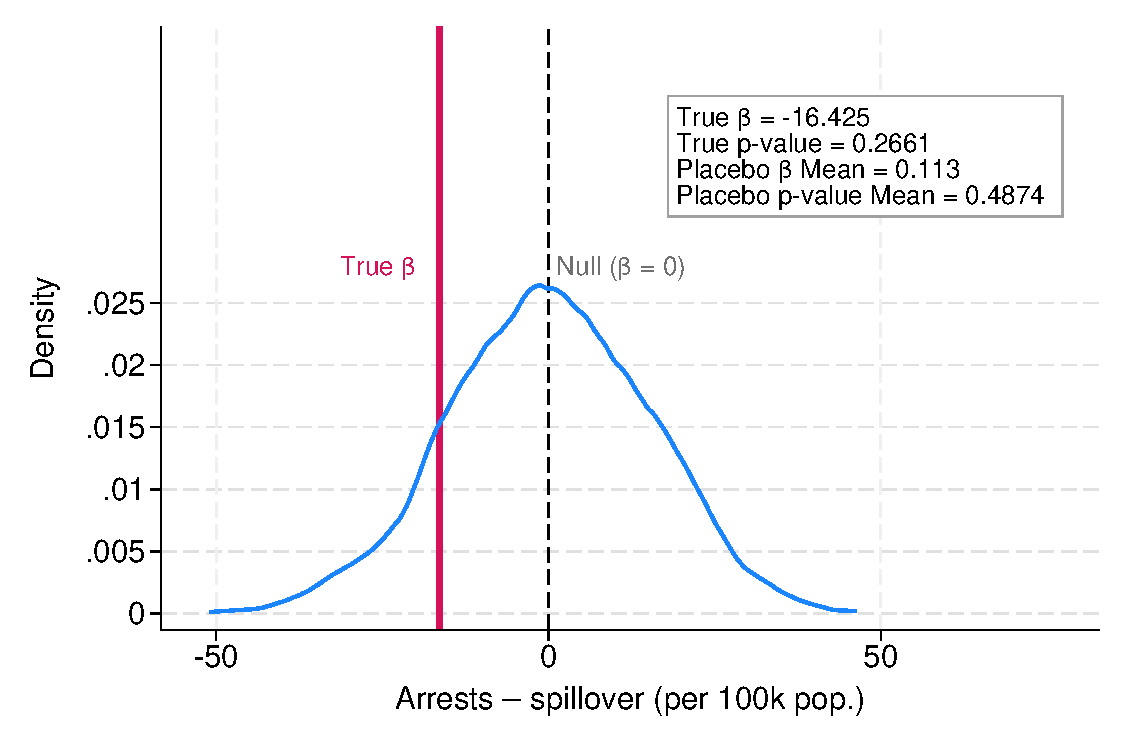
\includegraphics[width=\textwidth]{../manuscript/Graphs/CHDH_RI_placebo_arrests_spillover.pdf}
        \caption{Spillovers on Arrests}
        \label{fig:ri_arrests_spillover}
    \end{subfigure}
    \begin{minipage}{0.95\textwidth}
    \footnotesize
    Notes: This figure presents randomization inference results under the sharp null of no treatment effect, using the heterogeneity-robust estimator of \citet{Chaisemartin}. Each curve is the kernel density of 1{,}000 placebo ATT estimates obtained by jointly permuting \emph{Plan Cuadrante} adoption dates and never-treated status across municipalities (drawing from the empirical distribution of (date, status) pairs, so the marginal counts of treated and never-treated municipalities are preserved in every permutation). In each permutation the variable PC is shuffled across all 346 municipalities and a new time-varying treatment indicator is computed before re-estimating the dynamic effects. The solid colored vertical line marks the point estimate from the true rollout; the dashed black line marks the null expectation $\beta = 0$. The boxes report the true point estimate, its asymptotic two-sided $p$-value, and the mean of the placebo $\beta$ and placebo $p$-value distributions.
    \end{minipage}
\end{figure}
